\documentclass{article}

\usepackage{graphicx}
\usepackage[margin=0.5in]{geometry}
\usepackage{amsmath}
\usepackage{amssymb}
\usepackage[T1]{fontenc}
\usepackage{listings}
\usepackage{psfrag}
\usepackage{alltt}
\usepackage{rotating}

\pagenumbering{gobble}


\begin{document}

\begin{sidewaysfigure}[h!]
\centering
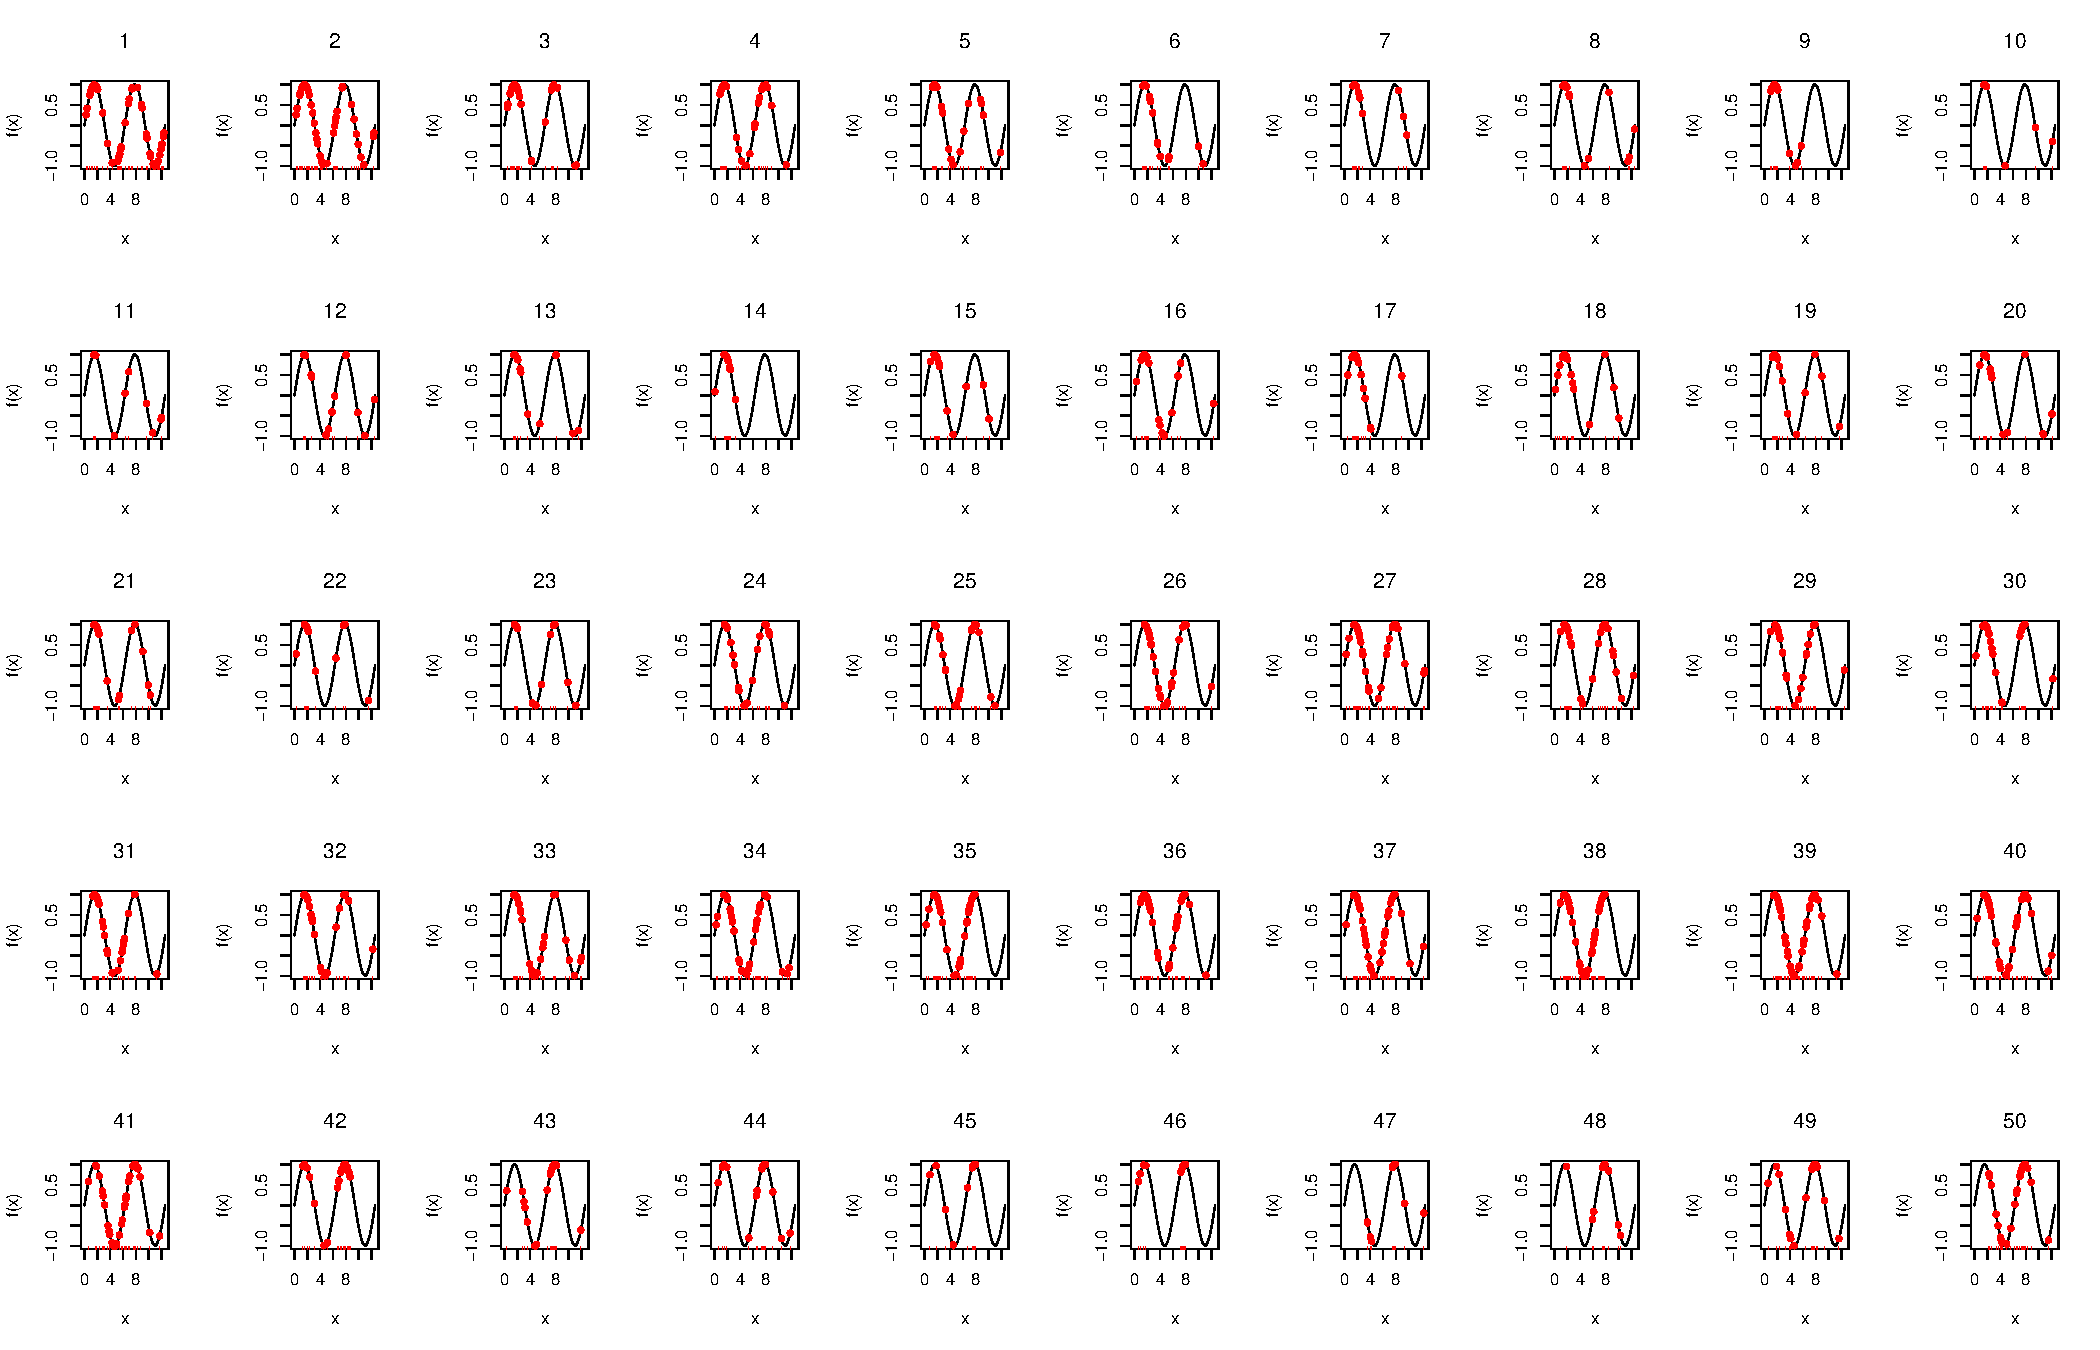
\includegraphics[width=1.0\textwidth]{gaSearchingR.pdf}
\end{sidewaysfigure}

\clearpage

\begin{sidewaysfigure}[h!]
	\begin{center}
		\begin{minipage}[h!]{0.7\textwidth}
			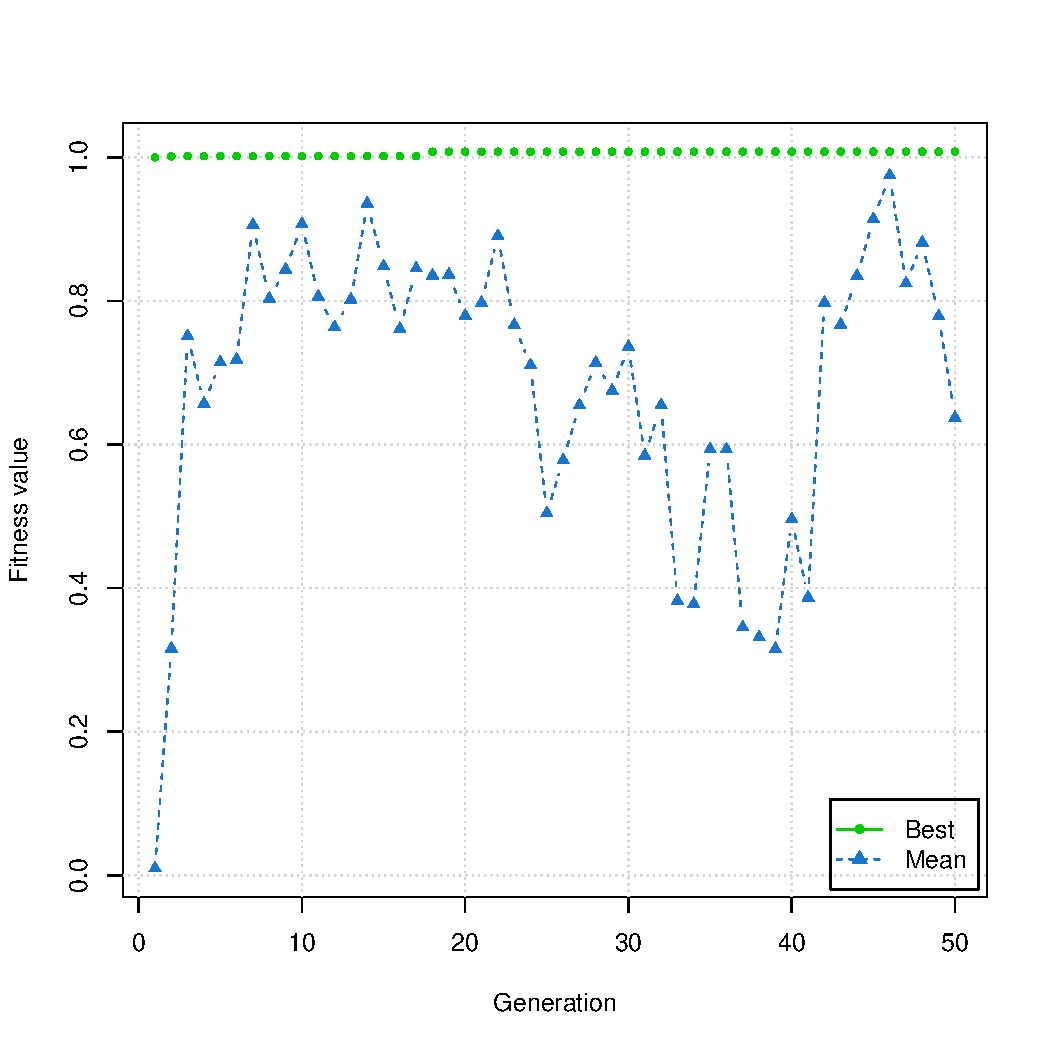
\includegraphics[width=\textwidth]{gaConvergeR.pdf}
		\end{minipage}
		\begin{minipage}[h!]{0.29\textwidth}
			\begin{alltt}
			+-----------------------------------+
			|         Genetic Algorithm         |
			+-----------------------------------+
			
			GA settings: 
			Type                  =  real-valued 
			Population size       =  50 
			Number of generations =  50 
			Elitism               =   
			Crossover probability =  0.8 
			Mutation probability  =  0.1 
			Search domain 
			          x1
			Min  0.00000
			Max 12.56637
			
			GA results: 
			Iterations             = 50 
			Fitness function value = 1.007854 
			Solution               = 
			           x1
			[1,] 7.854718
			\end{alltt}
		\end{minipage}
	\end{center}
\end{sidewaysfigure}

\clearpage

\begin{sidewaysfigure}[h!]
\centering
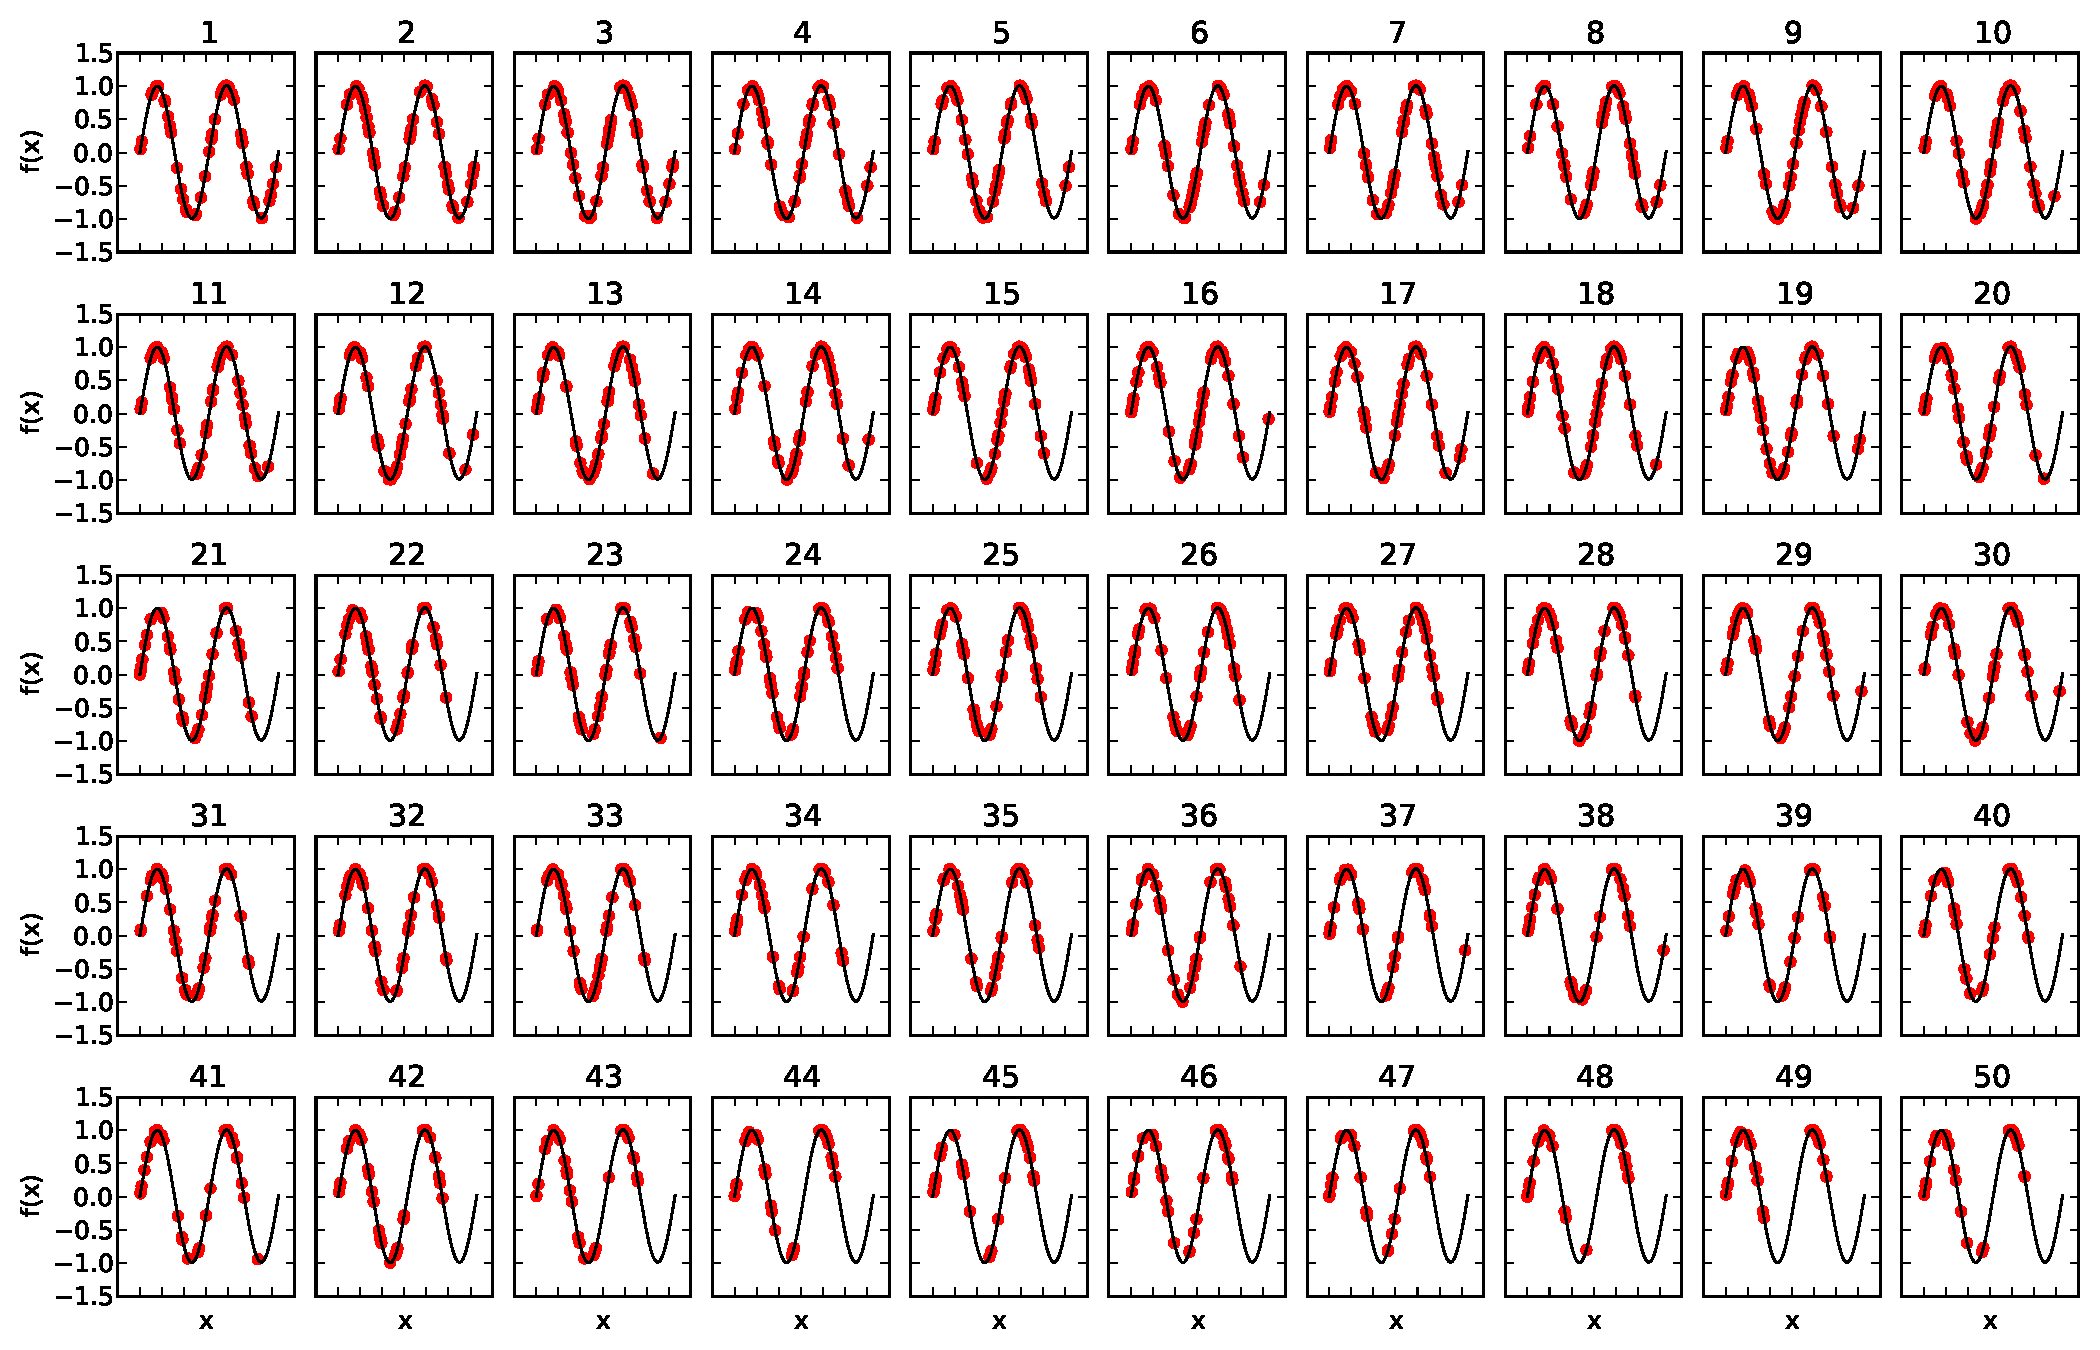
\includegraphics[width=1.0\textwidth]{gaSearchingMe.pdf}
\end{sidewaysfigure}

\clearpage

\begin{sidewaysfigure}[h!]
        \begin{center}
                \begin{minipage}[h!]{0.7\textwidth}
                        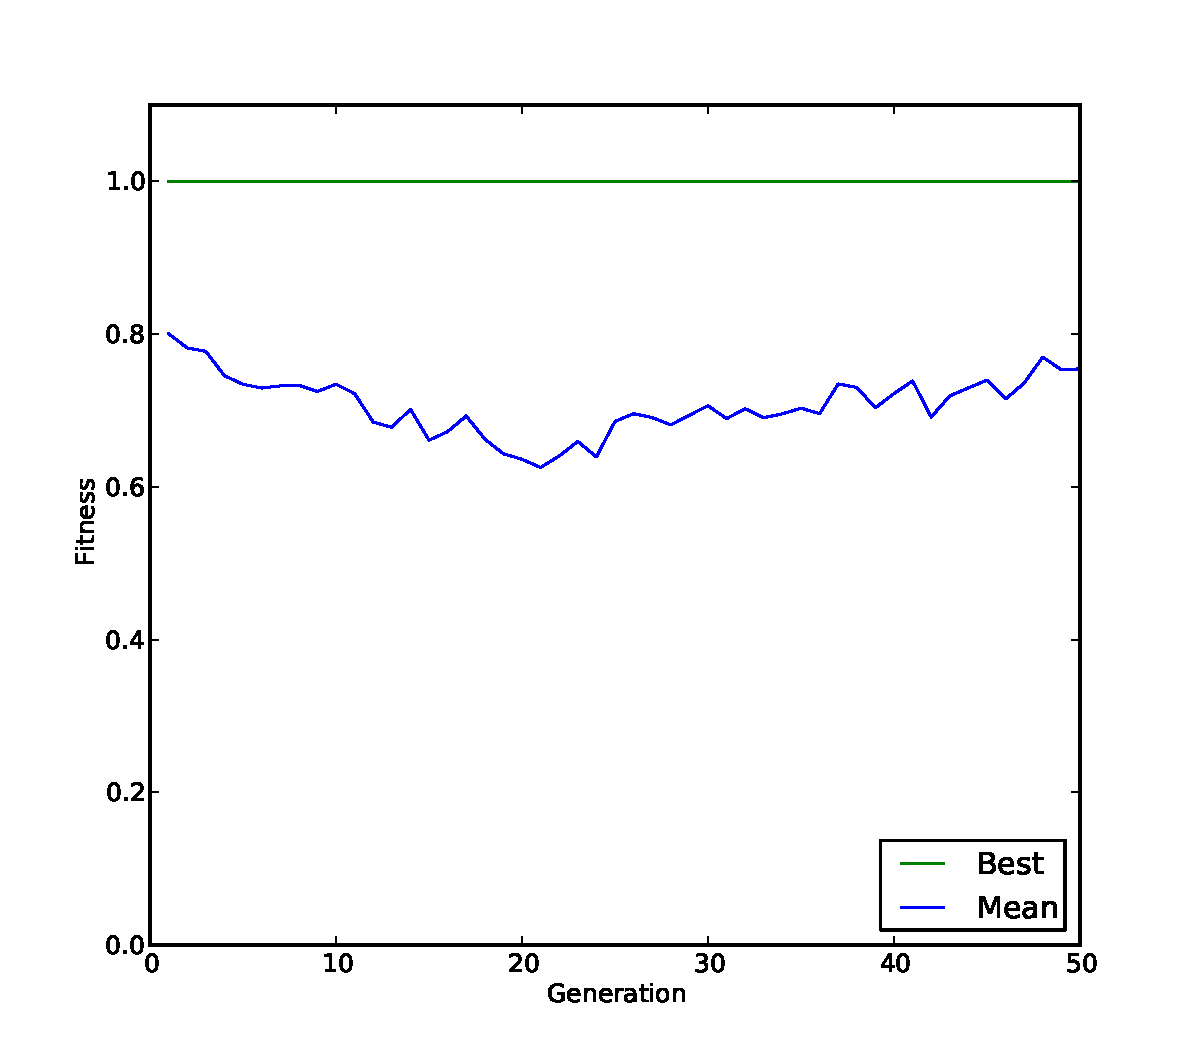
\includegraphics[width=\textwidth]{gaConvergeMe.pdf}
                \end{minipage}
                \begin{minipage}[h!]{0.29\textwidth}
                        \begin{alltt}
			      My Genetic Algorithm
			________________________________
			
			Population Size       = 50
			Number of Generations = 50
			Crossover Probability = 0.20
			Search Domain: [0.00, 12.57]
			Precision             = 2
			
			            Results  
			________________________________
			
			Fitness               = 1.007842
			argmax                = 7.86
                        \end{alltt}
                \end{minipage}
        \end{center}
\end{sidewaysfigure}

\clearpage


\begin{sidewaysfigure}[h!]
	\begin{center}
		\begin{minipage}[h!]{0.2\textwidth}
			\begin{alltt}
				My Outputs:
				Guess      = 2.000000
				Par        = 1.571796
				Value      = 1.001571
				Iterations = 50
				Hessian    = -1.000089			
			\end{alltt}
		\end{minipage}
		\begin{minipage}[h!]{0.19\textwidth}
			\begin{alltt}
				Optim Outputs:
				$par
				[1] 1001133
				
				$value
				[1] 1002.133
				
				$counts
				function gradient 
				       2        1 
				
				$convergence
				[1] 0
				
				$message
				NULL
				
				$hessian
				           [,1]
				[1,] -0.9999992
			\end{alltt}
		\end{minipage}	
		\begin{minipage}[h!]{0.6\textwidth}
			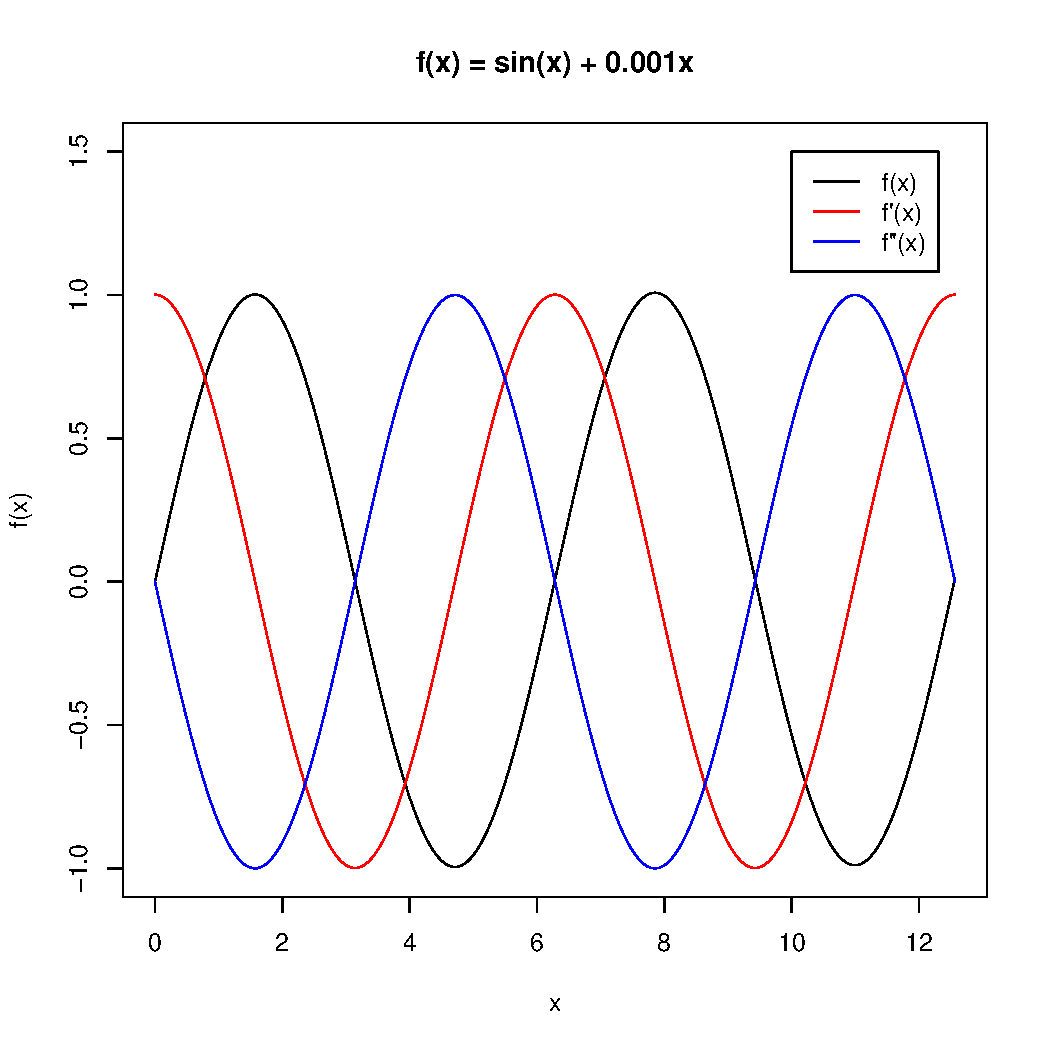
\includegraphics[width=\textwidth]{triggy.pdf}	
		\end{minipage}			
	\end{center}
\end{sidewaysfigure}

\clearpage

\begin{sidewaysfigure}[h!]
        \begin{center}
                \begin{minipage}[h!]{0.16\textwidth}
                        \begin{alltt}
				My Outputs:
				Guess      = -2.000000
				Par        = -0.666667
				Value      = 0.148148
				Iterations = 50
				Hessian    = -2.000011
          
                        \end{alltt}
                \end{minipage}
                \begin{minipage}[h!]{0.16\textwidth}
                        \begin{alltt}
				Optim Outputs:
				$par
				[1] -0.6666668
				
				$value
				[1] 0.1481481
				
				$counts
				function gradient 
				       3        1 
				
				$convergence
				[1] 0
				
				$message
				NULL
				
				$hessian
				          [,1]
				[1,] -2.000001
                        \end{alltt}
                \end{minipage}
		\begin{minipage}[h!]{0.16\textwidth}
                        \begin{alltt}
					My Outputs:
				Guess      = 0.000000
				Par        = -0.000001
				Value      = 0.000000
				Iterations = 50
				Hessian    = 2.000003 
                        \end{alltt}
                \end{minipage}
                \begin{minipage}[h!]{0.16\textwidth}
                        \begin{alltt}
				Optim Outputs:
				$par
				[1] -5.000001e-07
				
				$value
				[1] 2.5e-13
				
				$counts
				function gradient 
				       5        1 
				
				$convergence
				[1] 0
				
				$message
				NULL
				
				$hessian
				         [,1]
				[1,] 1.999997		
                        \end{alltt}
                \end{minipage} 
		 \begin{minipage}[h!]{0.16\textwidth}
                        \begin{alltt}
				My Outputs:
				Guess      = 2.000000
				Par        = -0.000001
				Value      = 0.000000
				Iterations = 50
				Hessian    = 2.000003
                        \end{alltt}
                \end{minipage}
                \begin{minipage}[h!]{0.16\textwidth}
                        \begin{alltt}
				Optim Outputs:
				$par
				[1] -5.000001e-07
				
				$value
				[1] 2.5e-13
				
				$counts
				function gradient 
				       5        1 
				
				$convergence
				[1] 0
				
				$message
				NULL
				
				$hessian
				         [,1]
				[1,] 1.999997
                        \end{alltt}
                \end{minipage}
        \end{center}
\end{sidewaysfigure}

\clearpage

\begin{sidewaysfigure}[h!]
	\begin{center}
		\begin{minipage}[h!]{0.49\textwidth}
			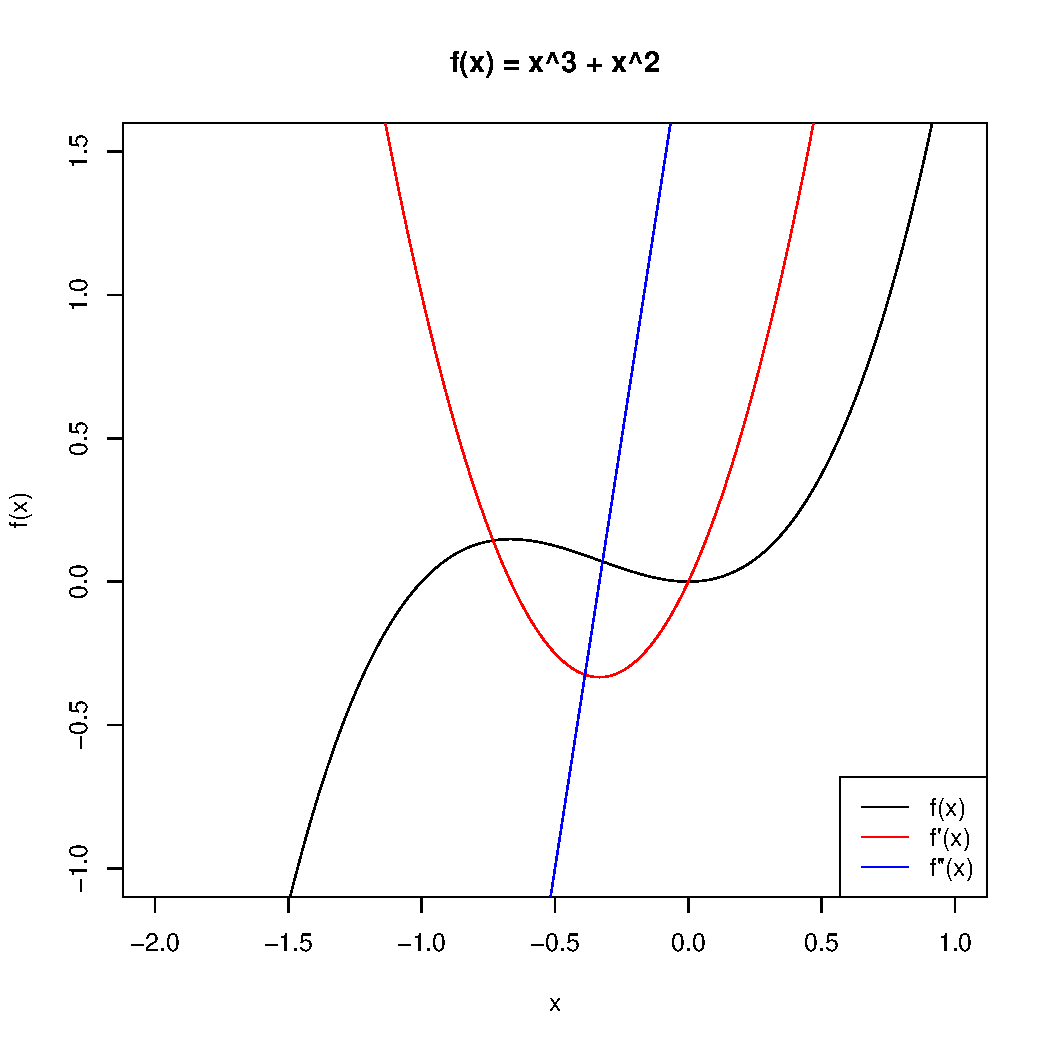
\includegraphics[width=1.0\textwidth]{poly32.pdf}
		\end{minipage}
		\begin{minipage}[h!]{0.49\textwidth}
			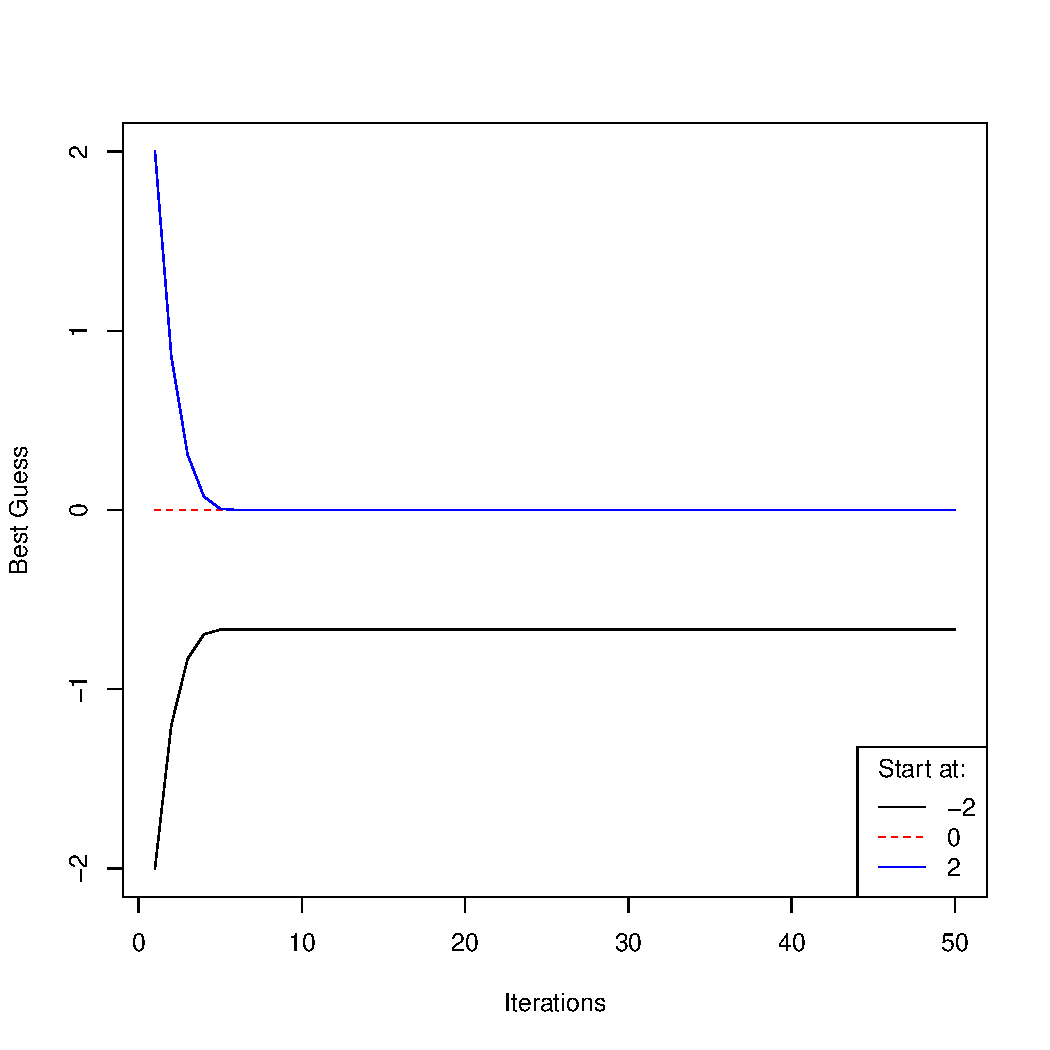
\includegraphics[width=1.0\textwidth]{gradConvergePoly32.pdf}
		\end{minipage}
	\end{center}
\end{sidewaysfigure}


\end{document}


%\begin{figure}[h!]
%              \begin{center}
%                \begin{minipage}[h!]{0.49\textwidth}
%                  \includegraphics[width=1.0\textwidth]{postSSbadThetaBadss.pdf}
%                \end{minipage}
%                \begin{minipage}[h!]{0.49\textwidth}
%                  \includegraphics[width=1.0\textwidth]{postTbadThetaBadss.pdf}
%                \end{minipage}
%              \end{center}
%\end{figure}
%
%\begin{sidewaysfigure*}[h!]
%        \includegraphics[width=10.2in, height=6in]{nGivenTrace.pdf}
%        \caption{The thinned (every $\thinning$ iterations) trace plot of the metropolis
%\end{sidewaysfigure*}
%
%\begin{alltt}
%+-----------------------------------+
%|         Genetic Algorithm         |
%+-----------------------------------+
%
%GA settings: 
%Type                  =  real-valued 
%Population size       =  50 
%Number of generations =  50 
%Elitism               =   
%Crossover probability =  0.8 
%Mutation probability  =  0.1 
%Search domain 
%          x1
%Min  0.00000
%Max 12.56637
%
%GA results: 
%Iterations             = 50 
%Fitness function value = 1.007854 
%Solution               = 
%           x1
%[1,] 7.854718
%\end{alltt}
%

